\section{Node Cognitive Architecture}
\label{sec:node}
%% ============================================================

The determinism partition (Section~\ref{sec:manifesto}) must be realized not only in the protocol but in the software a validator runs. A node that loaded a large language model into the same process as its consensus engine would have one careless code path away from letting nondeterministic model output influence a state root. We therefore prescribe a node architecture in which the cognitive machinery is physically separated from the consensus machinery by a process boundary and a firewall that only signed, structured artifacts may cross.

\subsection{The Sidecar Pattern}

A Thinking Chain validator is two processes, not one:

\begin{description}[style=nextline,leftmargin=0pt]
\item[The consensus node.] The deterministic core: it runs the EVM (including the Tier-1 inference precompile, which is pure integer code in-process and therefore safe), validates and produces blocks, maintains state, and verifies receipts via Pattern B. It contains \emph{no} large model and makes \emph{no} network call to a model during block execution. Its execution is a pure function of committed inputs (Theorem~\ref{thm:bridge}).
\item[The cognitive sidecar.] A separate process (or pool of processes) that hosts Tier-2 models (the \Hanzo{} engine, Section~\ref{sec:twotier}), performs off-chain generation when this node is a sampled provider, computes commit hashes, and reveals responses. The sidecar may be GPU-bound, nondeterministic, and as heavy as the operator likes; it never touches consensus state directly.
\end{description}

The two communicate only through the cognitive economy's message types (Section~\ref{sec:economy}): the sidecar learns of tasks it was sampled for by reading committed \AChain{} state, and it influences state only by submitting commit/reveal transactions that are settled by \SCC{} and verified like any other. The process boundary makes the partition a deployment fact, not merely a coding convention: even a buggy sidecar cannot inject a value into the consensus node's state root, because the only channel between them is the same committed-transaction channel any external party uses.

\subsection{The Signer Firewall}

The most sensitive component is the validator's signing key, which attests to blocks and (if the node is a provider) to cognitive responses. The \emph{signer firewall} is a strict rule about what that key will sign:

\begin{principle}[Signer firewall]
\label{prin:firewall}
A validator's signer signs only (i) canonical block attestations over deterministic state, and (ii) canonical, finite cognitive artifacts (commits and reveals over a declared output space). It never signs free-form model output, never signs a value it has not type-checked against a declared schema, and never signs on behalf of the cognitive sidecar without the sidecar's response having passed the finite-output and commit-binding checks. The firewall sits between the sidecar and the key: model output reaches the key only after being reduced to a finite, schema-valid, operator-bound artifact.
\end{principle}

The firewall is the local enforcement of the global finite-output rule (Principle~\ref{prin:finite}). Its purpose is to ensure that even a compromised or hallucinating sidecar cannot get the validator's key to sign something outside the finite output space---the worst a bad sidecar can do is cause its own commit to be wrong (and thus its own reveal to fail, slashing only itself), never to forge a signature over arbitrary content. Combined with operator-bound commits (Section~\ref{sec:scc}), the firewall ensures a node is accountable for exactly what it signed and nothing more.

\subsection{Node Topology}

Figure~\ref{fig:node} shows the validator. The consensus node and sidecar are separate failure domains: the sidecar can crash, be upgraded, swap models, or run on entirely separate hardware (even a separate machine, or the federated multi-vendor backends used for training) without affecting the consensus node's ability to validate and produce blocks. A validator that runs no sidecar at all is still a complete consensus participant---it simply earns no Tier-2 provider rewards. This graceful degradation is a direct consequence of the partition: cognition is an opt-in earning role layered on top of a consensus node, not a requirement of running one.

\begin{figure}[h]
\centering
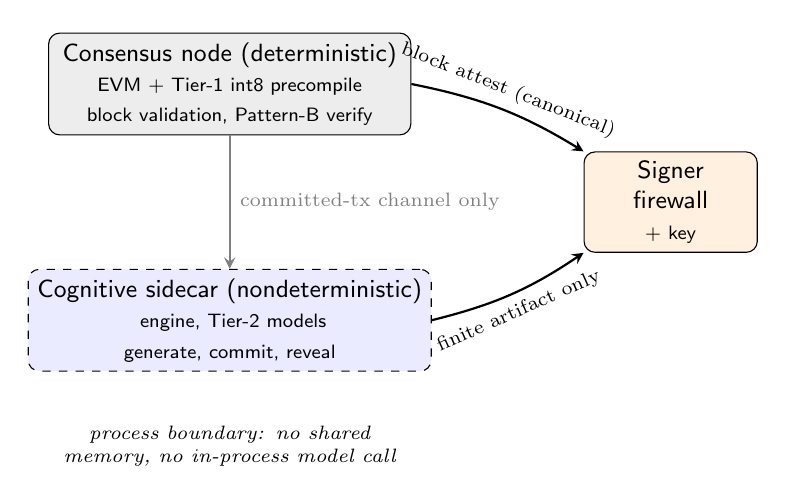
\begin{tikzpicture}[
    box/.style={rectangle, rounded corners, draw, align=center, font=\small\sffamily, minimum height=1cm},
    det/.style={box, fill=black!7, minimum width=4.6cm},
    cog/.style={box, fill=blue!8, dashed, minimum width=4.6cm},
    key/.style={box, fill=orange!12, minimum width=2.2cm},
    a/.style={->, thick, >=stealth}
]
\node[det] (cn) at (0,0) {Consensus node (deterministic)\\\scriptsize EVM + Tier-1 int8 precompile\\\scriptsize block validation, Pattern-B verify};
\node[cog] (sc) at (0,-3) {Cognitive sidecar (nondeterministic)\\\scriptsize \Hanzo{} engine, Tier-2 models\\\scriptsize generate, commit, reveal};
\node[key] (fw) at (5.6,-1.5) {Signer\\firewall\\\scriptsize + key};

\draw[a] (cn.east) to[bend left=10] node[above,sloped,font=\scriptsize]{block attest (canonical)} (fw.north west);
\draw[a] (sc.east) to[bend right=10] node[below,sloped,font=\scriptsize]{finite artifact only} (fw.south west);
\draw[a, gray] (cn) -- node[right,font=\scriptsize]{committed-tx channel only} (sc);
\node[font=\scriptsize\itshape, text width=4.4cm, align=center] at (0,-4.6) {process boundary: no shared memory, no in-process model call};
\end{tikzpicture}
\caption{Validator topology. The consensus node (deterministic, holds the Tier-1 integer precompile in-process) and the cognitive sidecar (nondeterministic, holds Tier-2 models) are separate failure domains communicating only over the committed-transaction channel. The signer firewall (Principle~\ref{prin:firewall}) admits only canonical block attestations and finite, schema-valid cognitive artifacts to the signing key.}
\label{fig:node}
\end{figure}

%% ============================================================
